\documentclass[12pt,a4paper]{article}
\usepackage[utf8]{inputenc}
\usepackage{amsmath}
\usepackage{amsfonts}
\usepackage{amssymb}
\usepackage{graphicx}

\title{Real-Time UML Embadded Systems Summary (page: 127-141)}

\begin{document}

\maketitle

\section{Problem 5.3 Apply Real-World Items and Physical Devices Strategies}
These two strategies are related in the sense that they seek to identify objects and
classes that represent things that exist in the physical world. The real-world items strategy seeks to identify objects from the real world that have information or resource that must be managed int the system. \\
 For instance: In a banking system, the customer is an object in the real world and we must maintain about information. (Name, Adress, Tax, etc).
 \\ \\
The Physical Devices Strategies identifies physical devices which are part of the system. (not external devices) The best way is not to model all physical devices that the system must monitor and control. A hardware is only
an actor if it is not integrated with the software into a shipped system.

\section{Problem 5.4 Apply Key Concepts and Transaction Strategies}
The Key Concepts strategy is the opposite of the real-world items strategy. It seeks
to find the essential concepts of a domain of discourse, particularly when these elements are abstractions and have no physical manifestation. \\ 
For instance: An account in a banking system is an abstract element.
 \\ \\
 
A transaction is the reification of an interaction (among objects) into an object itself. The interaction has a lifetime and persists until the transaction is completed. \\
For instance:  A withdrawal from a bank account is a transactional object. A request for an elevator to go to a particular floor is also a transactional object because it must be remembered until the elevator actually arrives at the floor.

\section{Problem 5.5 Apply Identify Visual Elements and Scenarios Strategies}
In systems with nontrivial user interfaces, these strategies often
work well together, because one of the issues that arises when considering scenarios that involve the human users of the system is how the user interfaces gather and provide information to the internal parts of the system that must deal with and respond to that information. \\

Scenario strategy the easiest way to construct a verifiably working
collaboration of classes to realize a use case. \\ Simply start with a use-case scenario. The use case will have a (possibly large) number
of scenarios as exemplars, illustrating examples of the use case unfolding as specific messages or events come in to the system. We will simply
elaborate object roles to show how the scenario unfolds at the object. In small systems (like RTLC) system-level use cases are used while in bigger system subsystem-level user cases are used. \\ \\
This elaboration is able to done in-line or by decomposition. In-line meaning: 
Copying the original scenario and starting adding object lifelines to the copy. The decomposition process is done by decomposing the lifeline into a more detailed scenario. 
\\
During the object-level scenario elaboration, you should uncover objects, services and parameters.
For creating service performed somewhere inside the system, you should ask yourself the following questions:
\begin{itemize}
\item What object has the information necessary to perform this service?
\item What object has the proper interfaces necessary to perform this service?
\item What object has the responsibility to perform this service?
\end{itemize}


You should add objects, services, and relations to detail this scenario. You might start at the beginning of the scenario, or somewhere in the middle—perhaps at a very important part of the use case or some part that you feel you can handle well. As you add objects to the scenario, you should add relevant classes to a class diagram, filling in the operation calls and event receptions to handle the message, attributes. \\

The first picture and second illustrate how this elaboration takes place. The first shows the high-level interaction. The lifeline in the middle is the use case, but it can just as easily be the “System” or another high-level object. The point is that
this element internally contains parts (typed by classes) that interact to provide the high-level behavior shown. \\\\

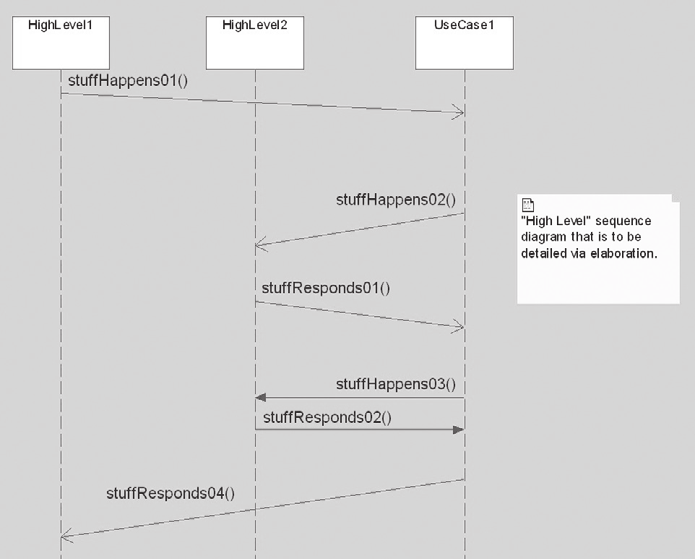
\includegraphics[scale=0.5]{high_level_seq.png} \\\\
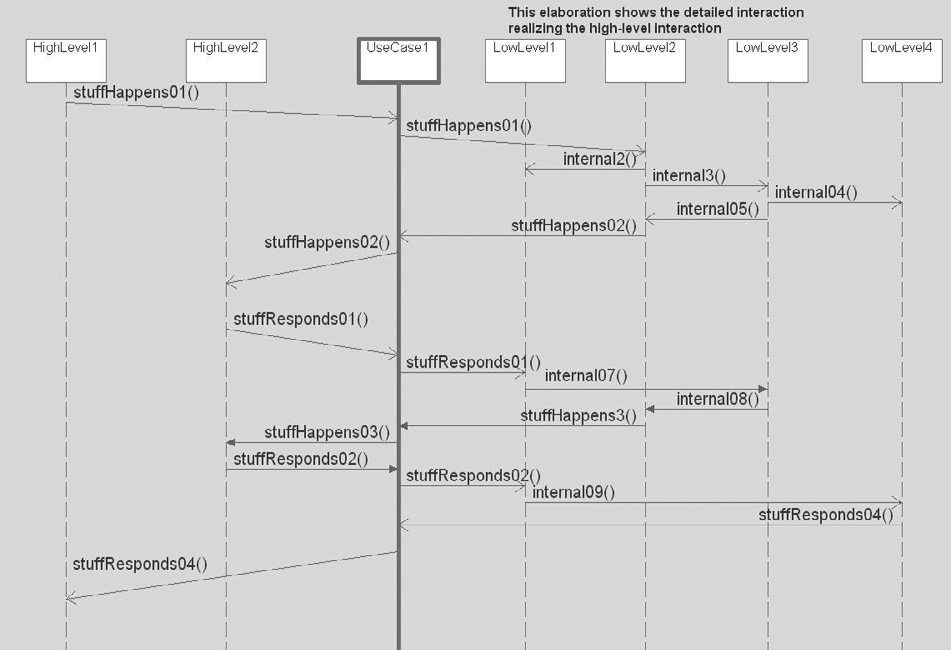
\includegraphics[scale=0.5]{elaborated_seq.png} \\\\\

At first impression, the Detect Vehicle use case does not seem to be an ideal case study for this strategy. The “scenario” consists of a single message “vehicleDetect” from the vehicle to the system but use-case scenario should never be a single message so it should be modeled too. The configuration of the detectors should be part of the scenarios.The lanes can be configured separately or all at once. There is a special “sentinel value” for the laneID that configures or enables all the detectors at once. if the laneId or the sensitivity provided is out of range the invalid
command is discarded and the previous settings are returned to the operator.\\
Consideration operator violates the constraints could be another scenario. 
\\\\
The radar detector is the only active emitter.
\\\\
As far as the human interface goes, the external UI has already been planned out and provided in the requirements specification.
\\\\


\section{Problem 5.6 Merge Models from the Various Strategies}
In this problem, you should merge together the different models that
have arisen from the application of the different strategies. The models would be most likely incrementally constructed by taking what is already added and adding objects, classes, relations, and features identified in additional strategies. The resulting use-case collaborations should be shown on a single
class (or structure) diagram for each system \\ \\

For the Roadrunner Traffic Light Control system, we have worked on two different use cases, Fixed Cycle Time Mode and Detect Vehicle. The system includes the elements that collaborate to realize both these use cases.  These use-case collaborations have been shown as two independent class diagrams and they will
continue to be shown in that way. The reason is that to scale the use of modeling techniques to real-world problems,
we must have some criteria for deciding what goes on which diagrams. If we maintain the diagrams as independent, then each maintains the purity of its purpose. \\ \\

The CUAV is a larger scale system, so we’ve narrowed our focus onto a single use case (Acquire Image) for a specific subsystem (Reconnaissance Management). One can imagine teams of people working independently, possibly in different areas of
the world, to develop the use cases for their own subsystems.

Finally, for both sample problems, answer the following questions:
\begin{itemize}
\item Which strategy worked best for you, and why?
\item Which strategy worked the least well for you, and why?
\item Did some strategies seem to be better identifying elements in one problem or the
other? Can you generalize that so that you know when to apply which strategies?
\item What combination of strategies do you think will be most effective for you?
\end{itemize}

\section{Looking Ahead}
We have used a number of different strategies to identify the “essential” or “analysis” objects and classes. These strategies are only partially orthogonal. In practice, the application of two or more strategies is required to identify all of the objects in the analysis model. For instance: A microwave oven had better have a microwave emitter, a track manager requires the notion of a track, and a navigation system needs the concepts of position, flight plan, and way-point to do its job.\\

The analysis model exactly corresponds to the idea of a platform independent model in the OMG’s model-driven architecture (MDA).It is devoid of The objects, classes, attributes, operations,
and relations identified may be optimized in many different ways using many different
design approaches with many different technology decisions to construct the
platform specific model design decisions. \\ 

While analysis is all about identifying elements required to meet the functional requirements, design is all about optimizing the analysis model to meet performance requirements and other design optimization criteria. Different optimization goals
or different technology selections result in different platform specific models from the same platform independent model. In this
way, the approach insulates you from technology churn and increases the interoperability of your system and its portability to new platforms. 
\\ \\
For systems that have a long life—such as military and aerospace systems—or systems that are part of product families and so have high reuse requirements, the MDA approach is both highly practical and effective.
\end{document} 